%!TEX root = ../../report.tex
\chapter{Long-term mapping in dynamic environments}
\label{long_term_mapping}
For a mobile robot to be able to function in an uncontrolled environment alongside other machines and humans, it is necessary for the robot to be able to sense and avoid the highly dynamic objects. All mobile robots navigating in such an area will have a system to handle these changes. Slower changes, however, that does not pose an immediate problem for the navigation of the environment are often disregarded. This is seen in the fact that often, a the map of the environment is only generated once and then used for an extended period of time. The assumption is that the surroundings does not change apart from the highly dynamical objects that should not be included in the map. This assumption can become increasingly flawed as time progressed due to the fact that most real world scenarios are not perfectly static. In an office, furniture might be moved around and in industrial settings, machines might be put up, or moved, or pallets stored in an area. As the discrepancy between the robot's internal representation and the actual environment increases, so does the chance for errors in localization or navigation. In order to overcome this, it is necessary for the robot to continue the process of mapping its environment as it navigates through it.
%
\section{Characteristics in industrial environments}
\label{sec:characteristics_in_industrial_environments}
An investigation of an representative industrial area where mobile robots are used, shows that areas share common dynamical characteristics. 
During a visit at SCAN A/S, a high degree of structure and fixed routines where observed. 
Different work stations produce different parts of the product, and place them in areas for the next station to continue on them.
Part of the production line at SCAN A/S, where a MIR robot is used, are shown in figure \ref{fig:scan-mir}. 
The machine is fixed to the floor and is almost as static as the walls in the factory.
Figure \ref{fig:scan-semi-static-obstacles} shows product parts that have been processed by one station, and are ready to be picked up by the next station. 
It might be possible to take advantage of the fixed routines and steady production rate, when building and updating a long term map.
As seen in the figure, objects are only roughly placed and are not aligned carefully, which can influence mapping with a high resolution grid.

\begin{table}[htbp]
	\caption{Regions of industrial environments}
	\label{tab:regions_of_industrial_environments}
	\begin{center}
		\begin{tabular}{p{2.cm} | p{2.6cm} | p{2.6cm} | p{2.6cm} | p{2.6cm}}
			\toprule
			\textbf{Type} & \textbf{Dominated areas} & \textbf{Object types} & \textbf{In navigation} & \textbf{In localization} \\ 
			\rowcolor[gray]{0.925}
			\textit{Highly dynamic} & Central corridors & Humans, moving vehicles & Avoid these areas if convenient & Consider avoiding this area \\
			\textit{Semi-static} & Temporary Storage areas & Pallets with parts or products & Incorporate for next planning with non-lethal & Landmarks value based on degree of dynamics \\ 
			\rowcolor[gray]{0.925}
			\textit{Static} & The rest & Walls, heavy machinery & Incorporate in map with lethal & Very good landmark \\			
			\bottomrule
		\end{tabular} 
	\end{center}
\end{table}

The areas can roughly be classified based on dynamics of the obstacles that are usually contained within them, as shown in table \ref{tab:regions_of_industrial_environments}. Areas with objects that moves almost constantly like humans are categorized as \textit{highly dynamic}, whereas areas with objects like walls, that never move are categorized as \textit{static}. The remaining \textit{semi-static} objects can be everything from parked vehicles to stored production parts, that moves with minutes or weeks in between. 

\begin{figure}[htbp]
	\centering
	\begin{subfigure}[t]{0.6\textwidth}
		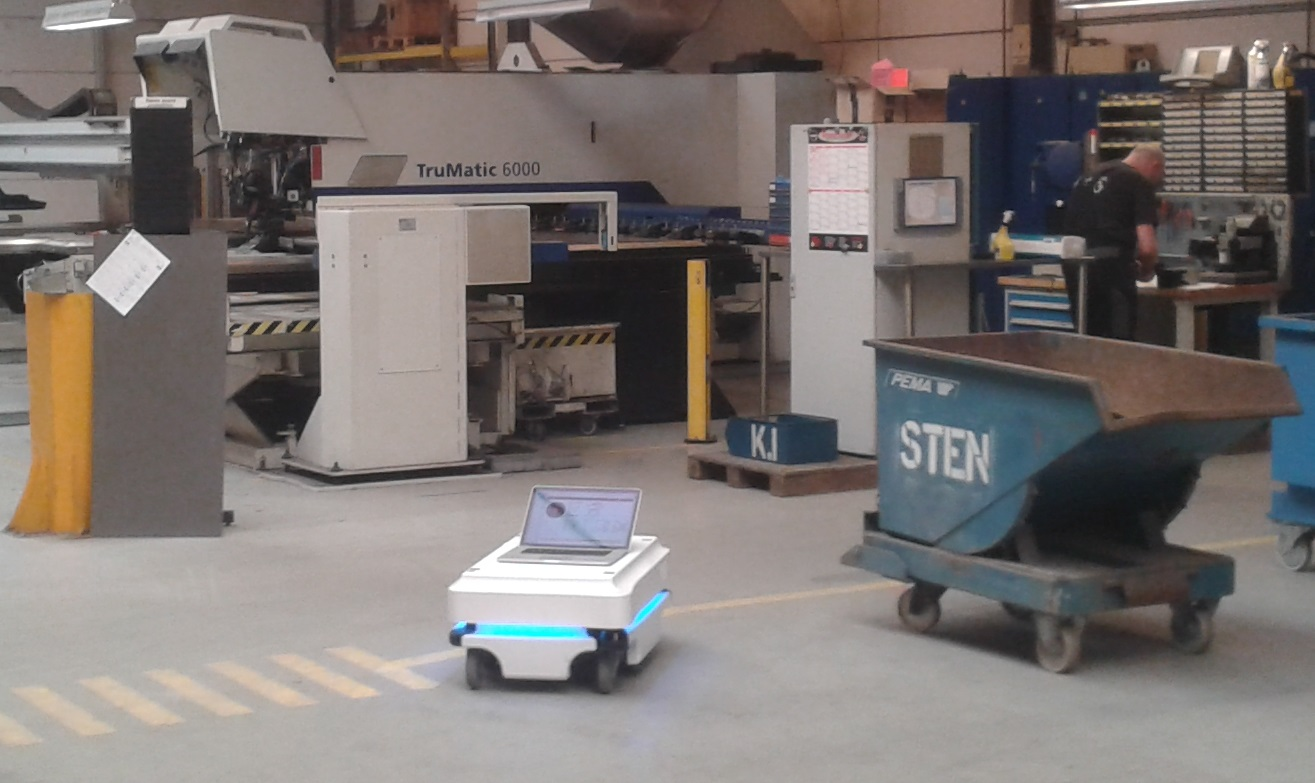
\includegraphics[width=1.0\textwidth]{chapters/mapping_of_dynamic_areas/figures/scan-mir}	
		\caption{MiR-100 robot navigating close to heavy machinery.}
		\label{fig:scan-mir}
	\end{subfigure}
	\begin{subfigure}[t]{0.3875\textwidth}
		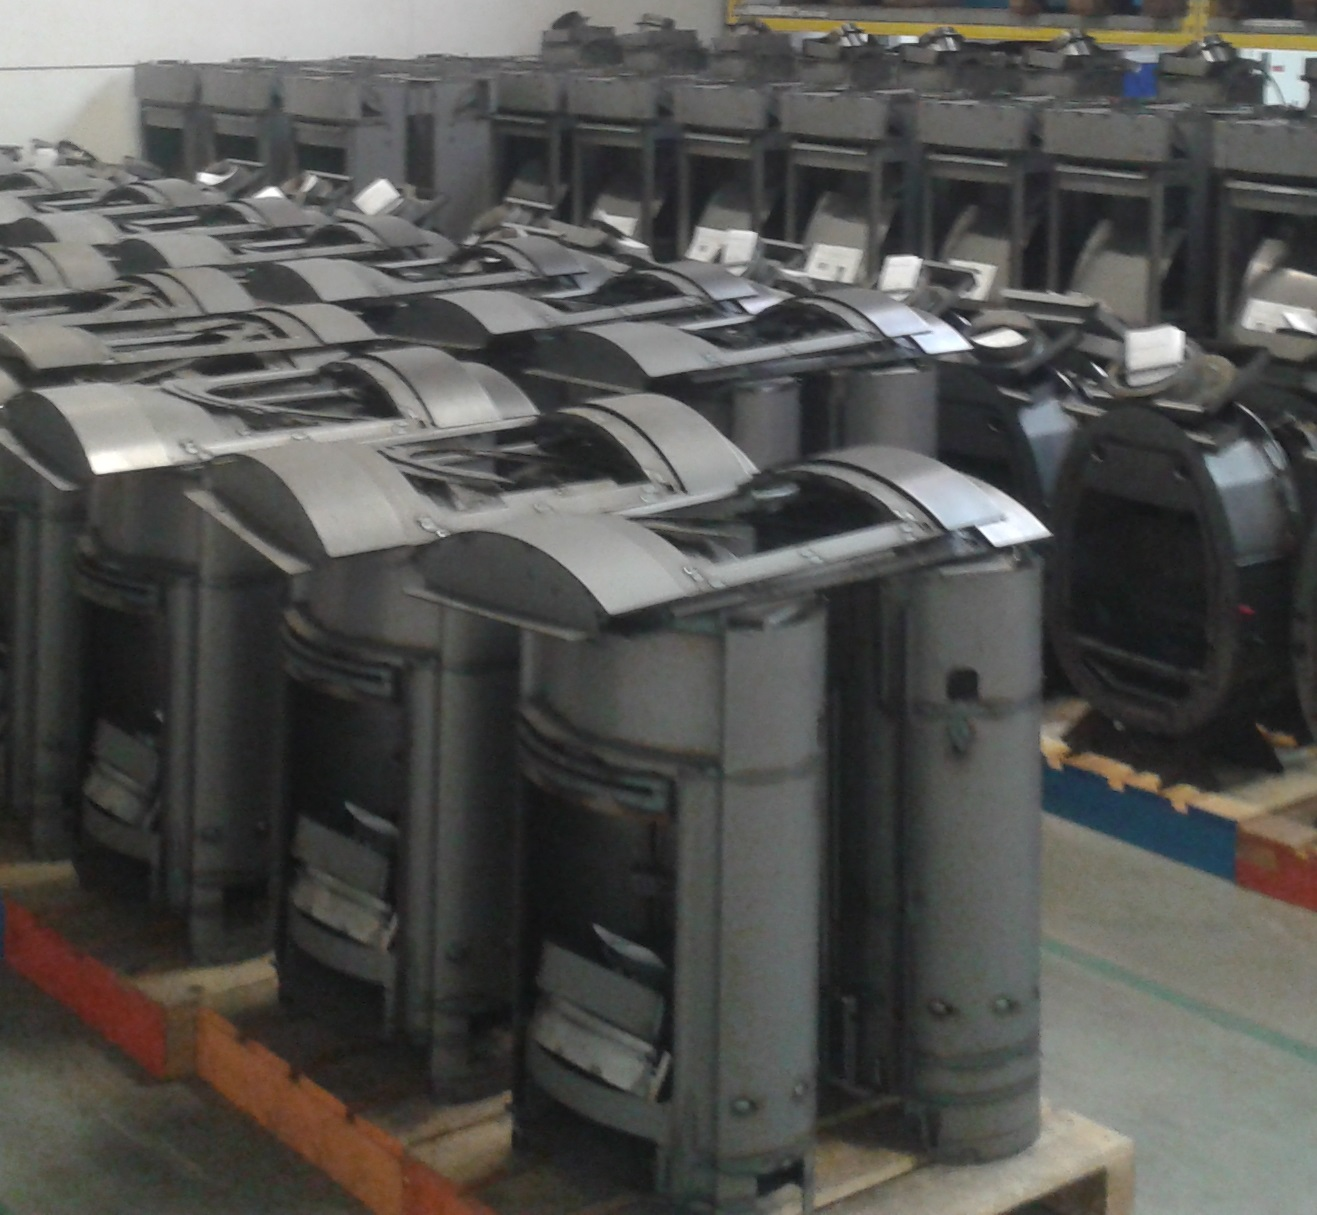
\includegraphics[width=1.0\textwidth]{chapters/mapping_of_dynamic_areas/figures/scan-semi-static-obstacles}
		\caption{\textit{Semi-static} obstacles in the form of product parts.}
		\label{fig:scan-semi-static-obstacles}
	\end{subfigure}
	\caption{Examples of obstacles in the production area at SCAN A/S.}
\end{figure}

The information of these areas can be incorporated in the representation of the world to avoid having to re-plan a path and to improve localization. 

The \textit{highly dynamic} objects should not be considered as obstacles, but some re-planning of the path might be unavoidable due to them. 
It is beneficial to include \textit{semi-static} obstacles in path planning to avoid having to re-plan, but by assigning them as lethal obstacles it might be impossible to plan a path although one is possible.
The \textit{static} objects should always be present as lethal obstacles when path planning to avoid navigating along obscure routes.

The \textit{highly dynamic} objects should not be included as landmarks for the localization, since they are moving almost constantly. 
Since the value of the \textit{semi-static} obstacles as landmarks depends on how dynamic they are, they should be weighted in the localization algorithm accordingly. 
The \textit{static} obstacles are very good landmarks.

If the \textit{semi-static} obstacles moves at a constant rate, it might be possible to predict the presence of it in the future by learning its transient behavior.
It is reasonable to assume a rather constant rate of movements of the production parts, since they are produced at approximately fixed rates and placed in confined areas.
By predicting the presence of obstacles it is possible to plan around them and use them as landmarks, when they are present.
This would be a huge improvements, but during the visit at SCAN A/S it became clear that obstacles are not placed exactly the same place, which complicates the learning process with a grid representation.
\section{Navigation in Dynamic Environments}
Mobile robot navigation is often done based on a costmap of the environment. This map represents the world as a grid of cells with associated costs. This cost is used to direct the search towards goal, along the path with the lowest cost. When the map is inconsistent with the environment, the robot might into a dead end. This necessitates re-planning, thus wasting time. Because the map is never updated the robot might continue to plan into the same dead end, making the system inefficient and annoy users. By updating the costmap with the dynamic mapping system, it is possible to reduce the amount of these errors.
\section{Localization with Static Map in Dynamic Environments}
Mobile robot localization is traditionally done based on a static map of the environment. This map is used to match up with the current LIDAR scans. A widely used system for this is the Monte Carlo localization \cite{probRob}. 
With Monte Carlo localization the sensor noise is assumed independent between consecutive time steps \cite{probRob}. This is violated when dynamic obstacles are present. Since the fact that if one measurement was too short, i.e. shorter than it should be by the static map, the next measurement in the same direction a small time later is also likely to be too short. Too short measurements indicates that, given the location of the robot’s sensors and the location of obstacles in the map, the measurement was shorter than the distance between the sensor and an obstacle. This violation stems from the unmodeled dynamics in the representation of the world. The effects of unmodeled dynamic obstacles in the world can be mitigated by detecting and removing hits on these obstacles from the observations used in the localization \cite{tang2015approach}\cite{fox1998position}. Methods for handling it this way is typically meant to reduce the effect of highly dynamical object but as they do not change the internal map, they do not improve localization as the static features in the world changes. Updating the internal map in order to incorporate the changes in the world to improve the localization is one of the tasks for dynamic learner. 

\section{Long-term SLAM in dynamic environments}
A possible solution to handling the changes in the world is continuously running a SLAM algorithm. 
These algorithms are often used to generate the initial map of the environment but continuing to run them will generate maps that are up-to-date and can encompass the changes in the world. The challenges in using a SLAM approach is associating parts of the newly generated map with previously obtained map. 
As the world might have changed between the SLAM runs any discrepancy can either be caused by an error in localization or a change in the environment. 
The problem of data association and the errors it can lead to is described in [REF HMM Lifelong LOC]. 
Another issue with running SLAM algorithms throughout the operation time is the memory and computational requirements of these algorithms. Using a multi-hypothesis SLAM algorithm a complete map for each hypothesis is required. This can become a problem when the area of operation becomes large. 
In order for the slam algorithms to generate good scan matching results the speed of the robot is important. If the speed is too high the quality of the map generated might be lowered. It is not desirable to limit the speed of the robot when it is performing its tasks. 



